%%%%%%%%%%%%%%%%%%%%%%%%%%%%%%%%%%%%%%%%%
% Medium Length Professional CV
% LaTeX Template
% Version 2.0 (8/5/13)
%
% This template has been downloaded from:
% http://www.LaTeXTemplates.com
%
% Original author:
% Rishi Shah 
%
% Important note:
% This template requires the resume.cls file to be in the same directory as the
% .tex file. The resume.cls file provides the resume style used for structuring the
% document.
%
%%%%%%%%%%%%%%%%%%%%%%%%%%%%%%%%%%%%%%%%%

%----------------------------------------------------------------------------------------
%	PACKAGES AND OTHER DOCUMENT CONFIGURATIONS
%----------------------------------------------------------------------------------------

\documentclass{resume} % Use the custom resume.cls style
\usepackage{graphicx}
\usepackage[left=0.75in,top=0.6in,right=0.75in,bottom=0.6in]{geometry} % Document margins
\usepackage{ucs} 
\usepackage[utf8x]{inputenc} % Включаем поддержку UTF8  
\usepackage[russian]{babel}  % Включаем пакет для поддержки русского языка 
\newcommand{\tab}[1]{\hspace{.2667\textwidth}\rlap{#1}}
\newcommand{\itab}[1]{\hspace{0em}\rlap{#1}}
\name{Vasiliy Krasnov} % Your name
%\address{123 Pleasant Lane \\ City, State 12345} % Your secondary addess (optional)
\address{+7(925)881-15-75 \\ vasiliykrasnov43@gmail.com \\ github.com/diedino} % Your phone number and email
\begin{document}
%----------------------------------------------------------------------------------------
%	EDUCATION SECTION
%----------------------------------------------------------------------------------------
\begin{rSection}{Education}

{\bf School №2097, Moscow} \hfill {\em 2006-2017}
\\{\bf National Research University Higher School of Economics, Moscow} \hfill {\em 2017 - Present} 
\\ Bachelor of Software Engineering \hfill { Overall Percentage: 47.65 }
\\{\bf Coursera - Data Structures by University of California San Diego} \hfill {\em 2018} 
\\ Verify at coursera.org/verify/GWG6QV2JMV2S
\\{\bf Coursera - Algorithmic Toolbox by University of California San Diego} \hfill {\em 2018} 
\\ Verify at coursera.org/verify/ZZE5D72VERAS
\\{\bf СберУниверситет - Introduction to Hadoop} \hfill {\em 2022} 

%Minor in Linguistics \smallskip \\
%Member of Eta Kappa Nu \\
%Member of Upsilon Pi Epsilon \\


\end{rSection}

\begin{rSection}{Carrier Objective}
 To work for an organization which provides me the opportunity to improve my skills and knowledge to grow along with the organization objective.
\end{rSection}
%--------------------------------------------------------------------------------
%    Projects And Seminars
%-----------------------------------------------------------------------------------------------
\begin{rSection}{Projects}
{\bf Modelling and Visualisation of “Addiator” Type Mechanical Slide Adder}
\\The course project aims at designing and showing the main principles of mechanical add/subtract calculator.\\
Using technologies: C\#, WPF.
\\{\bf Android Application for Bookcrossing}\\
The course project aims at creating mobile application for "the practice of leaving a book in a public place to be picked up and read by others, who then do likewise".\\
Using technologies: Java, Android SDK, Spring for backend, SQLite.
\\{\bf Car Buy \& Sell Application with BD interaction }\\
The freelance project aims at creating desktop application for car dealer centre where user can change data in DB on graphic interface, all sql triggers happen programally.\\
Using technologies: Java, JavaFx, MySQL.
\\{\bf Application for filling personal data }\\
A project that helped transfer filled digital data to various reporting views (e.g. Excel, Word).\\
Using technologies: Java, Apache POI, Postgres.

\end{rSection}
%----------------------------------------------------------------------------------------
%	TECHNICAL STRENGTHS SECTION
%----------------------------------------------------------------------------------------

\begin{rSection}{Technical Strengths}

\begin{tabular}{ @{} >{\bfseries}l @{\hspace{6ex}} l }
Skills \ & Java, C\#, C++, MySQL, HTLM, CSS, Angular, Git, Unit testing, Hadoop, Kafka  \\
Software \& Tools & Tools by JetBrains, Android Studio, Latex \\
OS \ & Windows, Unix (in most Ubuntu) \\
\end{tabular}

\end{rSection}

%----------------------------------------------------------------------------------------
%	WORK EXPERIENCE SECTION
%----------------------------------------------------------------------------------------

\begin{rSection}{Work Experience}
{\bf IT GEO - Junior Java Developer - Russia, Moscow} \hfill {\em 09.2019-02.2020} 
\\ Java, Spring, Postgres, MongoDB, Cryptography Service Provider, ruToken \\
{\bf Luna Wealth - Junior-to-Middle Java Developer - Russia, Moscow} \hfill {\em 02.2020-09.2021} 
\\ Java, Spring, Postgres, Flyway, KDB, Docker, Gitlab CI/CD, RabbitMQ \\
{\bf Sber Big Data Department - Middle Java Developer - Russia, Moscow} \hfill {\em 10.2021-05.2022} 
\\ Java, Spring, Solr, Docker, Jenkins, Kafka \\
{\bf Partially inactive } \hfill {\em 06.2022 - present} 
\\
\end{rSection}


\begin{rSection}{Languages}

English - Intermediate \\
Russian - Mother Tongue


\end{rSection}


%----------------------------------------------------------------------------------------
% Extra Curricular
%----------------------------------------------------------------------------------------
\begin{rSection}{Extra-Cirrucular} \itemsep -3pt
\item Member RosbankTech.Madness
\item Member MLH Hack in Russia
\item HanabiHack "Best case's solution"
%\item Trained and disciplined in National Cadet Corps (NCC), IIT Kanpur for a year.
 %\item  Participated in Vijyoshi Camp 2012 organized at Indian Institute of Science, Bangalore.
 %\item Won 2nd position in Kho-Kho in Intramurals conducted by Physical Education Section, IIT Kanpur.
 %\item Pursued French as second language during secondary school from Grade 6 to Grade 10. Also participated in French Song Competition and French G.K. Quiz in Class 10th. %

\end{rSection}
\begin{rSection}{Personal Traits}
\item Highly motivated to learn new things.
\item Ability to work as an individual as well as in group.
\end{rSection}
\begin{rSection}{My Photo}
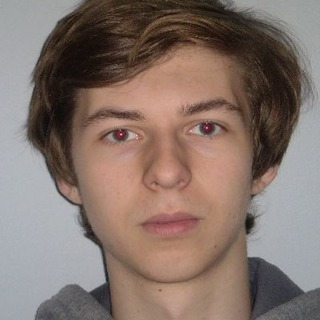
\includegraphics[scale = 0.5]{ya1.jpg}
\end{rSection}
\end{document}
